\documentclass{article}
\usepackage{listings}
\usepackage{mathrsfs}
\usepackage[utf8]{inputenc}
\usepackage{amssymb}
\usepackage{lipsum}
\usepackage{amsmath}
\usepackage{fancyhdr}
\usepackage{geometry}
\usepackage{scrextend}
\usepackage[english,german]{babel}
\usepackage{titling}
\setlength{\droptitle}{-3cm}
\usepackage{tikz}
\usepackage{algorithm,algpseudocode}
\usepackage[doublespacing]{setspace}
\usetikzlibrary{datavisualization}
\usetikzlibrary{datavisualization.formats.functions}
\usepackage{polynom}
\usepackage{amsmath}
\usepackage{gauss}
\usepackage{tkz-euclide}
\usetikzlibrary{datavisualization}
\usetikzlibrary{datavisualization.formats.functions}
\author{
Alexander Mattick Kennung: qi69dube\\
Kapitel 1
}
\usepackage{import}
\date{\today}
\geometry{a4paper, margin=2cm}
\usepackage{stackengine}
\parskip 1em
\newcommand\stackequal[2]{%
  \mathrel{\stackunder[2pt]{\stackon[4pt]{=}{$\scriptscriptstyle#1$}}{%
  $\scriptscriptstyle#2$}}
 }
\makeatletter
\renewcommand*\env@matrix[1][*\c@MaxMatrixCols c]{%
  \hskip -\arraycolsep
  \let\@ifnextchar\new@ifnextchar
  \array{#1}}
\makeatother
\lstset{
  language=haskell,
}
\lstnewenvironment{code}{\lstset{language=Haskell,basicstyle=\small}}{}
\usepackage{enumitem}
\setlist{nosep}
\usepackage{titlesec}

\titlespacing*{\subsection}{0pt}{2pt}{3pt}
\titlespacing*{\section}{0pt}{0pt}{5pt}
\titlespacing*{\subsubsection}{0pt}{1pt}{2pt}
\title{Vorlesung 4}


\begin{document}
	\maketitle
	zf: $\exists u ( t\to^* u ^*\gets s)$ dann ist t,s zf.\\
	konfluenz heißt, wenn es zwei ableitungsregeln gibt, die $t\to^* s$ und $t\to^* s'$ mit s, s' z.f (CHURCH ROSSER)\\
	lokale konfluenz nur einschritt entfernte ableitungen sind zf.(WCR)\\
	Newmanns lemma SN und lokal konfluent heißt TES global konfluent.\\
	kritisches Paar.\\
	Sei $l_1\to_0 r_1$ und $l_2\to_0 r_2$ $FV(l_1)\cap FV(l_2)=\emptyset$\\
	Weiterhin $l_1 = C(t)$ Definiere Term (t) und $C(\cdot)$ kontext, mit t nichttrivial (also nicht eine variable)\\
	und $\sigma = mgu(t,l_2)$.\\
	Dann heißt $(r_1\sigma, C(r_2)\sigma)$ kritisches Paar.\\
	Critical Pair Lemma. TES lokal konfluent $\iff$ alle kritischen Paare sind zf.\\
	Es gibt nur endlich viele kritische paare\\
	z.B.\\
	1) $x\cdot (y\cdot z)\to_0 (x\cdot y)\cdot z$\\
	2) $x\cdot x^{-1} \to e$\\
	ist das TES lokal konfluent?\\
	$l_1 = x\cdot (y\cdot z) $ $l_2 = x'\cdot (y'\cdot z')$, $t=x\cdot (y\cdot z)$, $C(\cdot)=(\cdot)$ $\sigma = [x'/x,y'/y,z'/z]$\\
	$(r_1\sigma, C(r_2)\sigma)=((x'\cdot y')\cdot z', (x'\cdot y')\cdot z')$\\
	``triviales kritischen Paar.''\\
	Dies entsteht bei kombination einer Regel mit sich selbst im $C(\cdot)=(\cdot)$\\
	$\implies$ triviale kritische Paare können ignoriert werden.\\
	$l_2 = x'\cdot (y'\cdot z')$\\
	$l_2 = x'\cdot (y'\cdot z')$, $C(t) = y\cdot z$ $C(\cdot)=x\cdot (\cdot)$, $\sigma = [x'/y, y'z'/z]$\\
	$l_1\sigma = x\cdot (x'\cdot(y'\cdot z')) = C(l_2)\sigma$\\
	$r_1\sigma = (x\cdot x')\cdot (y'\cdot z') = ((x\cdot x')\cdot y')\cdot z'$\\
	$C(r_2)\sigma = x\cdot ((x'\cdot y')\cdot z')\to (x(x'y'))z' = ((x\cdot x')\cdot y')\cdot z'$\\
	$\implies $ kritisches Paar ist zf.\\
	$l_1 =x(y\ z)$ und $(2) x\cdot x^{-1} \to_0 e$\\
	$l_2 = x'\cdot x'^{-1}$ $t=y\cdot z$ $C(\cdot)=x\cdot(\cdot)$, $\sigma = [x'/y, x^{'-1}/z]$\\
	$r_1\sigma = (xx')x^{-1'}$ $c(r_2) = x\cdot e$ ist nicht z.f.\\
	TES ist nicht lokal, somit auch nicht global konfluent.\\
	weiter Beobachtung:\\
	Bei n Regeln müssen $n^2$ kombinationen berücksichtigt werden. (ungeachtet versch. kontexte)\\
	Bei kritischen paaren, die auf verschiedenen Regeln basieren ($l_1\neq l_2$) m\textbf{uss mindestens 1 Funktionssymbol in $l_1$ und in $l_2$ vorkommen}.\\
	Bei kritischen Paaren, basierend auf der selben Regel muss mindestens ein funktionssymbol \textbf{mindestens 2 mal vorkommen}.\\
	\section{Übung 1}
	$l_1=A\cdot v$ ist kein kritisches Paar möglich, da entweder t trivial, oder $A=B$ oder $A=C$\\
	$l_1 =C\cdot (D\cdot x)$ $[t_1 = C\cdot (D\cdot w), t_2 = D\cdot w, t_3 = w]$\\
	Wieder kein kritisches paar möglich.\\
	$l_1 = B(x*y)$\\
	$l_2 = A*v$ $t=xy$ $C(\cdot) = B\cdot (\cdot)$ $\sigma =[A/x, v/y]$\\
	$l_1\sigma = B\cdot (A\cdot v)$\\
	$r_1\sigma = A\cdot (D\cdot A)$, $C(r_2)\sigma = B(B(CV))$\\
	$l_2 =C(D*w)$ $t=x*y, C(\cdot)=B\cdot (\cdot)$\dots (A*(DC), B(B(CW)))\\
	$l_2 =B(xy)$ $t=xy$ $C(\cdot), B\cdot(\cdot)$ $\sigma = [B/x, x'y'/y]$\\
	$l_2 = B*(B*Z)$ $t=B*(x*y), \sigma = [B/x,z/y]$ $(A\cdot (D\cdot B), D\cdot z)$\\
	$l_w = B*(B*z)$ $t=x*y$ $c(\cdot) = B\cdot (\cdot)$ $\sigma = B/x, B*z/y$\\
	$(A\cdot(D\cdot B), B\cdot(D\cdot Z))$\\
	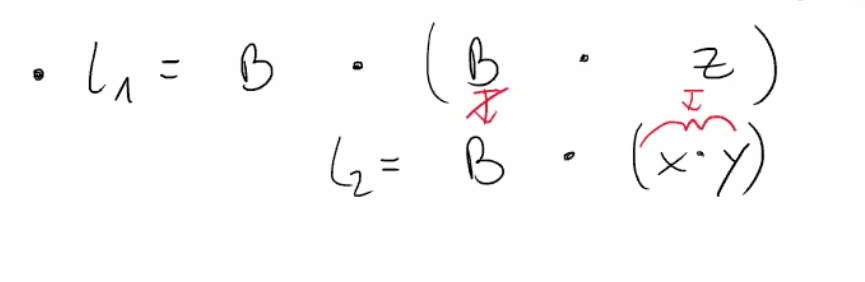
\includegraphics[width=128px]{kompaktesCriticalPair.png}
\end{document}